%%%%%%%%%%%%%%%%%%%%%%%%%%%%%%%%%%%%%%%%%%%% DOCUMENT CLASS %%%%%%%%%%%%%%%%%%%%%%%%%%%

\documentclass[12pt]{amsart}
%\documentclass[draft, 12pt]{amsart}


%%%%%%%%%%%%%%%%%%%%%%%%%%%%%%%%%%%%%%%%%%%%%%%%%% STANDARD PACKAGES %%%%%%%%%%%%%%%%%%%%%%%%%%%%%%%%%%%%%%%%%

\usepackage{amssymb,amsmath,amsthm,amscd,mathrsfs,graphicx, color}
\usepackage[cmtip,all,matrix,arrow,tips,curve]{xy}
\usepackage[notref,notcite]{showkeys}
%\usepackage[colorlinks]{hyperref}
\usepackage{multicol}
\usepackage{hyperref}
\usepackage[usenames,dvipsnames]{xcolor}
\hypersetup{colorlinks=true,citecolor=OliveGreen,linkcolor=BrickRed,urlcolor=BlueViolet}
\usepackage[active]{srcltx}
\usepackage{mathpazo}
\usepackage{setspace}\doublespacing 
%Double space, and make it easier for the grader to grade your homework.
%\usepackage{fullpage} 
%Use wide margins, and make it easier for the grader to grade your homework.


%%%%%%%%%%%%%%%%%%%%%%%%%%%%%%%%%%%%%%%%%%%%%% TIKZ FOR GRAPHING %%%%%%%%%%%%%%%%%%%%%%%%%%%%%%%%%%%%%%%%%%%%%%%%%%%%%%%
\usepackage{tikz,pgfplots}


%%%%%%%%%%%%%%%%%%%%%%%%%%%%%%%%%%%%%%%%%%%%%% 		ANSWER BOXES 		%%%%%%%%%%%%%%%%%%%%%%%%%%%%%%%%%%%%%%%%%%%
 \setlength\fboxsep{.3cm}
\setlength\fboxrule{.05cm}

\newcommand*{\boxedcolor}{red}
\makeatletter
\renewcommand{\boxed}[1]{\textcolor{\boxedcolor}{%
  \fbox{\normalcolor\m@th$\displaystyle#1$}}}
\makeatother

\makeatletter
\newcommand{\boxedred}[1]{\textcolor{red}{%
  \fbox{\normalcolor\m@th$\displaystyle#1$}}}
\makeatother

\makeatletter
\newcommand{\boxedblue}[1]{\textcolor{blue}{%
  \fbox{\normalcolor\m@th$\displaystyle#1$}}}
\makeatother




%%%%%%%%%%%%%%%%%%%%%%%%%%%%%%%%%%%%%%%%%%%%%%%%%%%% THEOREM ENVIRONMENTS %%%%%%%%%%%%%%%%%%%%%%%%%%%%%%%%


\numberwithin{equation}{section}
\newtheorem{teo}{Theorem}[section]
\newtheorem{pro}[teo]{Proposition}
\newtheorem{lem}[teo]{Lemma}
\newtheorem{cor}[teo]{Corollary}
\newtheorem{con}[teo]{Conjecture}
\newtheorem{convention}[teo]{}



\newtheorem{teoalpha}{Theorem}
\renewcommand{\theteoalpha}{\Alph{teoalpha}}
\newtheorem{proalpha}[teoalpha]{Proposition}
\newtheorem{coralpha}[teoalpha]{Corollary}


\theoremstyle{definition}
\newtheorem{dfn}[teo]{Definition}
\newtheorem{exa}[teo]{Example}
\newtheorem{que}[teo]{Question}

\theoremstyle{remark}
\newtheorem{rem}[teo]{Remark}
\newtheorem{nte}[teo]{Note}

%%%%%%%%%%%%%%%%%%%%%%%%%%%%%%%%%%%%%%%%%%%%%%% SOME CONDITIONALS FOR NOTES %%%%%%%%%%%%%%%%%%%%%%%%%%%%%%%%%%%

% Declare a new conditional
\newif\ifnotes
\notestrue 	% Show details
%\notesfalse 	% Exclude details


%%%%%%%%%%%%%%%%%%%%%%%%%%%%%%%%%%%%%%%%%%%%% COMMENTS %%%%%%%%%%%%%%%%%%%%%%%%%%%%

\newcommand{\marg}[1]{\normalsize{{\color{red}\footnote{{\color{blue}#1}}}{\marginpar[\vskip -.3cm {\color{BrickRed}\hfill\thefootnote$\implies$}]{\vskip -.3cm{ \color{BrickRed}$\impliedby$\thefootnote}}}}}

\newcommand{\qc}[1]{\marg{#1}}

%%%%%%%%%%%%%%%%%%%%%%%%%%%%%%%%%%%%%%%%%%%%%%%%%%% BEGIN DOCUMENT %%%%%%%%%%%%%%%%%%%%%%%%%%%%%%%%%%%
 
\begin{document}

\bibliographystyle{amsalpha}


%%%%%%%%%%%%%%%%%%%%%%%%%%%%%%%%%%%%%%%%%%%%%%%% AUTHOR INFO %%%%%%%%%%%%%%%%%%%%%%%%%%%%%%%%%%%% 

\author[QI]{QI WANG}
\address{University of Colorado, Department of Mathematics,  Campus Box 395,
Boulder, CO 80309-0395}
\email{casa@math.colorado.edu}
\date{\today}
%\thanks{I would like to take this opportunity to thank my class for their support.}


%%%%%%%%%%%%%%%%%%%%%%%%%%%%%%%%%%%%%%%%%%%%%%%% TITLE AND ABSTRACT %%%%%%%%%%%%%%%%%%%%%%%%%%%%%%%%%%%%

\title[Homework 2]{Homework 2 \\ \ \\  MATH 2001}

\begin{abstract} 
This is the second homework assignment.  The problems are from Hammack \cite[Ch.~1, \S 1.2]{H13}:
\begin{itemize}

\item \textbf{Chapter 1}  
\textbf{Section 2}, Exercises:  2, 4, 8, 12, 18.

\end{itemize}
\end{abstract}


\maketitle


\tableofcontents

%%%%%%%%%%%%%%%%%%%%%%%%%%%%%%%%%%%%%%%%%%%%%%%% HOMEWORK ASSIGNMENT %%%%%%%%%%%%%%%%%%%%%%%%%%%%%%%%%%%%

%%%%%%%%%%%%%%%%%%%%%%%%%%%%%%%%%%%%%%%%%%%%%%%%%%%%%%%%%%%%%%%%%%%%%%%%%%%%%%%%%%%%%%%%%% CHAPTER 1 %%%%%%%%%%%%%%%%%%%%%%%%%%%%%%%%%%%%%%%%%%%%%%%%%%%%%%%%%%%%%%%%%%%%%%%%%%%%%%%%%%%%%%%%%%%%%%%%%%%


%%%%%%%%%%%%%%%%%%%%%%%%%%%%%%%%%%%%%%%%%%%%%%%% SECTION 1.1 %%%%%%%%%%%%%%%%%%%%%%%%%%%%%%%%%%%%

\section*{Chapter 1 Section 1.2}


%%%%%%%%%%%%%%%%%%%%%%%%%%%%%%%%%%%%%%%%%%%%%%%% EXERCISE 2 %%%%%%%%%%%%%%%%%%%%%%%%%%%%%%%%%%%%

\subsection*{Ch.1, \S 1.2,  Exercise 2} Write out the indicated sets by listing their elements between braces. Suppose $A = \{\pi , e, 0\}$ and $B = \{0, 1\}$ .

\begin{enumerate}

\item[(a)] $A \times B$

\item[(b)] $B \times A$

\item[(c)] $A \times A$

\item[(d)] $B \times B$

\item[(e)] $\emptyset \times B$

\item[(f)] $(A \times B) \times B$

\item[(g)] $A \times (B \times B)$

\item[(h)] $B^3$

\end{enumerate}

\begin{proof}[Solution to Ch.1, \S 1.2,  Exercise 2] I worked with the entire class on this solution.
%\qc{You are encouraged to work together on homework assignments.  However, for each problem you must write your own solution, and, as I have done here,  you must indicate with whom you worked, and you must cite any resources you used in solving  the  problem.}

\begin{enumerate}

\item[(a)] 
$A \times B$ 
$$ =(\pi, 0), (\pi, 1), (\rm{e}, 0), (\rm{e}, 1), (0, 0), (0, 1) $$

\item[(b)]
$B \times A$
$$ =(0, \pi), (0, \rm{e}), (0, 0), (1, pi), (1, \rm{e}), (1, 0) $$

\item[(c)]
$A \times A$
$$ =(\pi, \pi), (\pi, e), (\pi, 0), (e, \pi),$$
$$ (e, e), (e, 0), (0, \pi), (0, e), (0, 0)$$

\item[(d)]
$B \times B$
$$ =(0, 0), (0, 1), (1, 0), (1, 1) $$

\item[(e)]
$A \times \emptyset$
$$ = \emptyset $$

\item[(f)]
$(A \times B) \times B$
$$ =((\pi, 0), 0), ((\pi, 0), 1), ((\pi, 1), 0), ((\pi, 1), 1), ((e, 0), 0), ((e, 0), 1), $$
$$((e, 1), 0), ((e, 1), 1), ((0, 0), 0), ((0, 0), 1), ((0, 1), 0), ((0, 1), 1)$$

\item[(g)]
$A \times (B \times B)$
$$ =(\pi, (0, 0)), (e, (0, 0)), (0, (0, 0)), (\pi, (0, 1)), (e, (0, 1)), (0, (0, 1)),$$
$$(\pi, (1, 0)), (e, (1, 0)), (0, (1, 0)), (\pi, (1, 1)), (e, (1, 1)), (0, (1, 1))$$

\item[(h)]
$A \times B \times B$
$$ =(\pi, 0, 0), (\pi, 0, 1), (\pi, 1, 0), (\pi, 1, 1), (e, 0, 0), (e, 0, 1), $$
$$(e, 1, 0), (e, 1, 1), (0, 0, 0), (0, 0, 1), (0, 1, 0), (0, 1, 1)$$


\end{enumerate}

\end{proof}


%%%%%%%%%%%%%%%%%%%%%%%%%%%%%%%%%%%%%%%%%%%%%%%% EXERCISE 8 %%%%%%%%%%%%%%%%%%%%%%%%%%%%%%%%%%%%


\subsection*{Ch.1, \S 1.2,  Exercise 4}  Write the following set by listing its elements between braces: 
$\{n \in \mathbb Z : 2 < n < 5 \} \times \{n \in \mathbb Z : |n| = 5 \}$.   


\begin{proof}[Solution to Ch.1, \S 1.2,  Exercise 4]
$$ A = \{n \in \mathbb Z : 2 < n < 5 \} $$
$$ A = \{3, 4\} $$
$$ B = \{n \in \mathbb Z : |n| = 5 \} $$
$$ B = \{5, -5\} $$
$$ A \times B = (3, 5), (3, -5), (4, 5), (4, -5) $$

%\begin{align*}
%x^3+5x^2=-6x &\iff x^3+5x^2+6x=0\\
%& \iff x(x^2+5x+6)=0\\
%& \iff x(x+2)(x+3)=0\\
%& \iff x=0, \text{ or } x=-2, \text{ or } x=-3.
%\end{align*}
\end{proof}


%%%%%%%%%%%%%%%%%%%%%%%%%%%%%%%%%%%%%%%%%%%%%%%% EXERCISE 18 %%%%%%%%%%%%%%%%%%%%%%%%%%%%%%%%%%%%


\subsection*{Ch.1, \S 1.2,  Exercise 8}  Write the following set by listing its elements between braces: 
$$ \{0, 1\}^4 $$



\begin{proof}[Solution to Ch.1, \S 1.2,  Exercise 8]
$$ \{0, 1\}^4 $$
$$ =(0, 0, 0, 0), (0, 0, 0, 1), (0, 0, 1, 0), (0, 0, 1, 1), $$
$$ (0, 1, 0, 0), (0, 1, 0, 1), (0, 1, 1, 0), (0, 1, 1, 1), $$
$$ (1, 0, 0, 0), (1, 0, 0, 1), (1, 0, 1, 0), (1, 0, 1, 1), $$
$$ (1, 1, 0, 0), (1, 1, 0, 1), (1, 1, 1, 0), (1, 1, 1, 1) $$

\end{proof}


%%%%%%%%%%%%%%%%%%%%%%%%%%%%%%%%%%%%%%%%%%%%%%%% EXERCISE 30 %%%%%%%%%%%%%%%%%%%%%%%%%%%%%%%%%%%%


\subsection*{Ch.1, \S 1.2,  Exercise12} Sketch these Cartesian products on the $x - y$ plane $ \mathbb R^2 $:
$$ [-1, 1] \times [0, 1] $$



\begin{proof}[Solution to Ch.1, \S 1.2,  Exercise 12]
\ \newline

\begin{center}

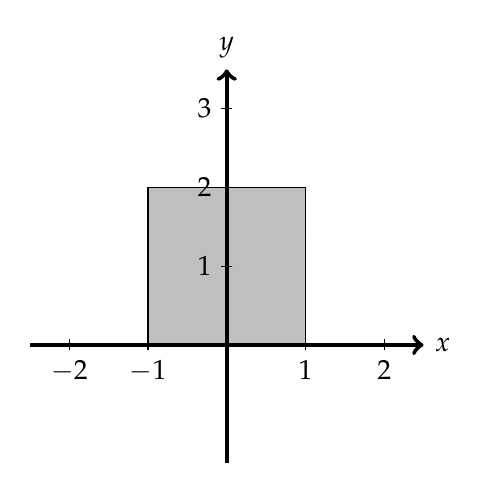
\begin{tikzpicture}

%graph
\draw[draw=gray!50!white, fill=gray!50!white]
	plot[smooth, samples = 100, domain = -1 : 1] (\x, {0}) --
	plot[smooth, samples = 100, domain = 1 : -1] (\x, {2});
\draw (-1, 0) -- (-1, 2) -- (1, 2) -- (1, 0);

%coordinate system
\draw[->, ultra thick] (-2.5, 0) -- (2.5, 0) node[right]{$x$};
\draw[->, ultra thick] (0, -1.5) -- (0, 3.5) node[above]{$y$};
\foreach \x in {-2, -1, , 1, 2}
	\draw (\x, 2pt) -- (\x, -2pt) node[below] {$\x$};
\foreach \y in { , 1, 2, 3}
	\draw (2pt, \y) -- (-2pt, \y) node[left] {$\y$};
	
\end{tikzpicture}

\end{center}

\end{proof}



%%%%%%%%%%%%%%%%%%%%%%%%%%%%%%%%%%%%%%%%%%%%%%%% EXERCISE 38 %%%%%%%%%%%%%%%%%%%%%%%%%%%%%%%%%%%%


\subsection*{Ch.1, \S 1.2,  Exercise 18} Sketch these Cartesian products on the $x - y$ plane $ \mathbb R^2 $:
$$ \mathbb{Z} \times \mathbb{Z} $$


\begin{proof}[Solution to Ch.1, \S 1.2,  Exercise 18]
\ \newline

\begin{center}

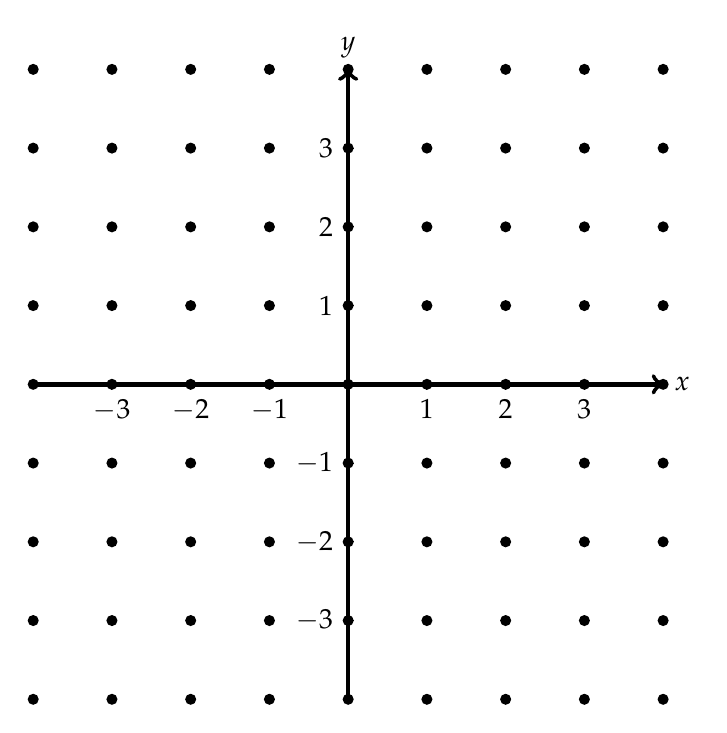
\begin{tikzpicture}

%graph
\foreach \x in {-4, ..., 4}
\foreach \y in {-4, ..., 4}
{
	\fill (\x, \y) circle (2pt);
}

%coordinate system
\draw[->, ultra thick] (-4, 0) -- (4, 0) node[right]{$x$};
\draw[->, ultra thick] (0, -4) -- (0, 4) node[above]{$y$};
\foreach \x in { -3, -2, -1, , 1, 2, 3}
	\draw (\x, 2pt) -- (\x, -2pt) node[below] {$\x$};
\foreach \y in { -3, -2, -1, , 1, 2, 3}
	\draw (2pt, \y) -- (-2pt, \y) node[left] {$\y$};
	
\end{tikzpicture}

\end{center}

\end{proof}



%%%%%%%%%%%%%%%%%%%%%%%%%%%%%%%%%%%%%%%%%%%%%%%% The End %%%%%%%%%%%%%%%%%%%%%%%%%%%%%%%%%%%%

\ \newpage

\ifnotes


\else
	This is not the full version.  This can be useful if there is scratch work you want to keep for yourself, but you do not want other people to see. 
\fi




\bibliography{templateHW}
\end{document}
